\section{Theorie}
\label{sec:Theorie}

\subsection{Spannung und Elastizitätsmodul}
Kräfte, welche an Oberflächen von elastischen Körpern angreifen, rufen Verformungen
hervor. Wird diese Kraft auf die Flächeneinheit bezogen, folgt daraus die
Spannung als physikalische Größe. Der senkrecht zur Oberfläche stehende Anteil der
Spannung heißt Normalspannung $\sigma$. Der Tangentialanteil heißt Schubspannung.

\begin{figure}[H]
  \centering
  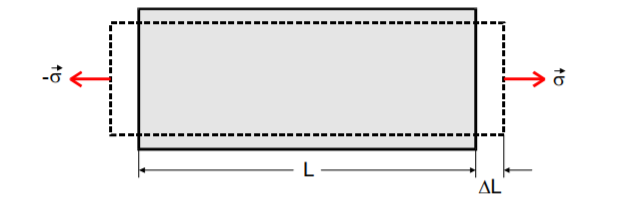
\includegraphics[height=5cm]{biegungbild1.PNG}
  \caption{Verformung eines Stabes durch eine Normalspannung. \cite{sample}}
  \label{fig:biegungbild1}
\end{figure}

Ist bei einer Verformung die relative Längenänderung $\frac{\Delta L}{L}$ hinreichend klein, so ist
bei den meisten Körpern ein linearer Zusammenhang zwischen
der Normalspannung $\sigma$ und $\frac{\Delta L}{L}$ Längenänderung der zu sehen:
\begin{equation}
  \sigma = E\frac{\Delta L}{L}
\end{equation}
Dies wird als Hook'sches bezeichnet. Der Proportionalfaktor $E$ ist
der Elastizitätsmodul und ist materialabhängig.

\subsection{Durchbiegung eines einseitig eingespannten Stabes}
Greift eine Kraft auf einen einseitig eingespannten Stab an, verformt er sich.
Die Längenänderungen eines Qerschnittes des Stabes ist nicht mehr konstant.

\begin{figure}[H]
  \centering
  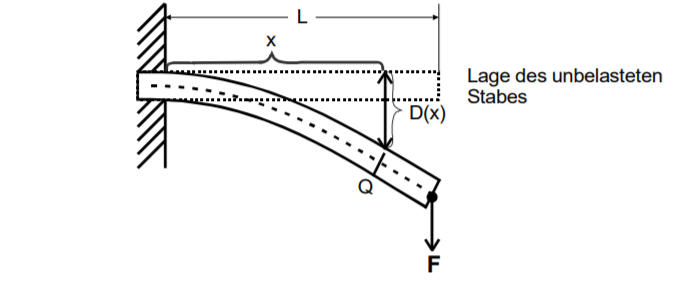
\includegraphics[height=5cm]{einseitigerstab.PNG}
  \caption{Verformung eines einseitig eingespannten Stabes. \cite{sample}}
  \label{fig:einseitigerstab}
\end{figure}

Die Durchbiegung $D(x)$ bezeichnet den Abstand eines Oberflächenpunktes des Stabes
in Ruhe von dem Punkt nach einer Verformung, wie Abbildung 2 zeigt. Die
gestrichelte Linie beschreibt die neutrale Faser, eine Fläche, welche sich durch die Verformung nicht ändert.
Die oberen Schichten werden gestreckt und die unteren gestaucht. Die Kraft $F$
übt im Abstand $L _ x$ ein Drehmoment $M_F$ auf den Querschnitt $Q$ aus. Verformt sich
der Probenkörper, entstehen im Innern, Normalspannungen, welche der Verformung
entgegen wirken. Im Gleichgewichtszustand stellt sich eine endliche Durchbiegung ein.
Die Zug- und Druckspannung, die an dem Querschnitt angreifen bewirken ein Drehmoment $M_{\sigma}$.
Dieses lässt sich durch Integration über $Q$ berechnen.
\begin{equation}
  M_{\sigma} = \int_Q y \sigma(y) \symup{d}q
\end{equation}

y bezeichnet den Abstand des Flächenelements $dq$ von der neutralen Faser.

\begin{figure}[H]
  \centering
  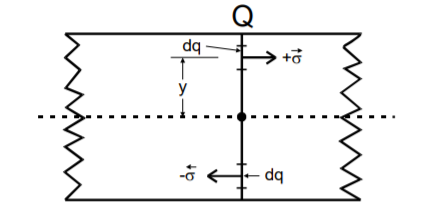
\includegraphics[height=5cm]{stabausschnitt.PNG}
  \caption{Flächenelement und Spannungen. \cite{sample}}
  \label{fig:stabausschnitt}
\end{figure}

An jeder Stelle $x$ sind die Drehmomente gleich.
\begin{equation}
  M_F =M_{\sigma}
\end{equation}

Mit dem Hebelarm $L-X$ gilt:
\begin{equation}
  M_F = F(L - x)
\end{equation}
Mit Gleichung (2) und Gleichung (3) folgt:
\begin{equation}
  \int_Q y \sigma(y) \symup{d}q = F(L - x)
\end{equation}

%$\sigma (y)$ lässt sich mit dem HooK'schen Gesetz berechnen.
%Für ein kurzes Stabstück $\Delta x$ gilt im Abstand y von der neutralen Faser:
%\begin{equation}
%  \sigma (y) = E \frac{\delta x}{\Delta x}
%\end{equation}
%$\delta x$ ist die Längenänderung von $\Delta x$ in Folge einer Verformung.
%
%\begin{figure}[H]
%  \centering
%  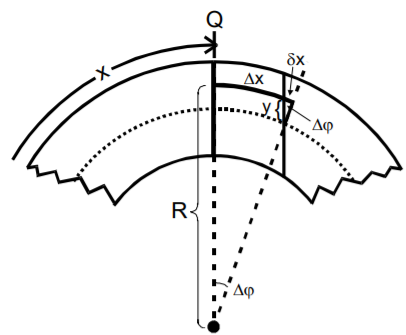
\includegraphics[height=5cm]{deltax.PNG}
%  \caption{Geometrische Beziehung zwischen $\delta x$, $\Delta\varphi$ und $R$. \cite{sample}}
%  \label{fig:deltax}
%\end{figure}
%
%In Abbildung 4 ist erkennbar, dass für $\delta x$ gilt:
%
%\begin{equation}
%  \delta x = y \Delta \varphi = y \frac{\Delta x}{R}
%\end{equation}
%
%$R$ ist der Krümmungsradius an der Stelle $x$. Für Gleichung (6) folgt:
%
%\begin{equation}
%  \sigma (y) = E \frac{y}{R}
%\end{equation}
Durch weitere geometrische Überlegungen folgt für kleine Krümmungen:
\begin{equation}
  E\frac{y}{\sigma(y)} \approx \frac{\symup{d}^2 D}{\symup{d} x^2}
\end{equation}

%Für Gleichung (8) folgt daraus:
%\begin{equation}
%  \sigma (y) = Ey \frac{\symup{d}^2 D}{\symup{d} x^2}
%\end{equation}

%Für Gleichung (8) folgt schließlich:
%\begin{equation}
%  E \frac{\symup{d}^2 D}{\symup{d} x^2} \int_Q y^2 \symup{d}q = F(L - x)
%\end{equation}

Für die Durchbiegung folgt daraus:
\begin{equation}
  D(x) = \frac{F_g}{2EI} \left(Lx^2 - \frac{x^3}{3} \right)
\end{equation}

Für $0 \leq x \leq L$. $F_G$ ist die Gewichtskraft. I ist das Flächenträgheitsmoment und ist definert durch:
\begin{equation}
  I = \int_Q y^2 \symup{d}q(y)
\end{equation}

Die Integrationskonstanten in Gleichung (11) verschwinden, da an der Einspannstelle
die Auslenkung und die Durchbiegung Null ist.

\subsection{Durchbiegung eines zweiseitig eingespannten Stabes}
Die Verformung eines Stabes, der zweiseitig eingespannt ist, ist in Abbildung 5
dargestellt.

\begin{figure}[H]
  \centering
  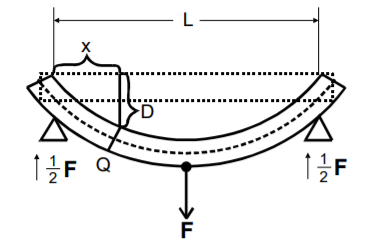
\includegraphics[height=5cm]{zweiseitig.PNG}
  \caption{Verformung eines zweiseitig eingespannten Stabes. \cite{sample}}
  \label{fig:zweiseitig}
\end{figure}

Die Kraft $\frac{F}{2}$ übt nun ein Drehmoment $M_F$ auf die Querschnittsfläche $Q$ aus.
Im Bereich $0 \leq x \leq \frac{L}{2}$ gilt für das Drehmoment:
\begin{equation}
  M_f = -\frac{F}{2}x
\end{equation}
Für den andren Bereich $\frac{L}{2} \leq x \leq L$ folgt dementsprechend:
\begin{equation}
  M_F = -\frac{F}{2}(L - x)
\end{equation}

Mit diesen Drehmomenten folgt für Gleichung (10) in dem Bereich $0 \leq x \leq \frac{L}{2}$:
\begin{equation}
  \frac{\symup{d}^2 D}{\symup{d} x^2} = - \frac{F}{EI}\frac{x^2}{2}
\end{equation}
Und für den Bereich $\frac{L}{2} \leq x \leq L$:
\begin{equation}
  \frac{\symup{d}^2 D}{\symup{d} x^2} = -\frac{1}{2} \frac{F}{EI}(L - x)
\end{equation}

Werden diese Gleichungen integriert lässt sich die Durchbiegung angeben. Es gilt:
\begin{align}
  D(x) &= \frac{F}{48EI} \left(3L^2x -4x^3 \right)   &\text{für}   &0 \leq x \leq \frac{L}{2} \\
  D(x) &= \frac{F}{48EI} \left(4x^3 -12Lx^2 + 9L^2x - L^3 \right)  &\text{für}   &\frac{L}{2} \leq x \leq L
\end{align}
